\documentclass[submit,noauthor]{ono}
% \documentclass[submit,techrep,noauthor]{ipsj}
%\documentclass{ipsj}
\usepackage[dvipdfmx]{graphicx}
\usepackage{graphicx}
\usepackage{float}
\usepackage{url}
\usepackage{lmodern}
\usepackage{booktabs}
% \usepackage[tablesfirst]{endfloat}
% \usepackage{endfloat}
\usepackage{tabularx}

\def\Underline{\setbox0\hbox\bgroup\let\\\endUnderline}
\def\endUnderline{\vphantom{y}\egroup\smash{\underline{\box0}}\\}
\def\|{\verb|}

\begin{document}

\title{IRDBデータによる日本の機関リポジトリの特徴の分析\\}

\etitle{Analysis of the characteristics of Japanese institutional repositories using IRDB data\\}

\paffiliate{JU}{東京大学駒場図書館\\
	Komaba Library, University of Tokyo}

\author{小野 亘}{Wataru, ONO}{https://orcid.org/0000-0002-6398-9317}[ono.wataru.plus@gmail.com]

\begin{abstract}
本稿は、Pythonのデータ解析のためのライブラリであるPANDASを用い、
NIIのIRDBデータから、日本の機関リポジトリの特徴の分析を行ったものである。
日本の機関リポジトリは、紀要に大きな特徴があることをデータの上から明らかにし、
特徴的な機関の抽出を行った。
\end{abstract}


\begin{jkeyword}
	IRDB, 機関リポジトリ, 紀要
\end{jkeyword}

\begin{eabstract}
This paper is an analysis of the characteristics of Japanese institutional
 repositories from NII's IRDB data using PANDAS, 
 a library for data analysis in Python.
 The data revealed that Japanese institutional repositories have 
 significant characteristics in their departmental bulletin paper (Kiyou), 
 and I extracted the characteristic institutions.
\end{eabstract}

\begin{ekeyword}
	IRDB, Intitutional repositories, Departmental Bulletin Paper
\end{ekeyword}

\maketitle

%1
\section{はじめに}

本稿では,国立情報学(NII)のIRDBから統計データを取得し、
日本の機関リポジトリに登録されたコンテンツの種別(資源タイプ)の分析を行い、
その側面から、日本の機関リポジトリの特徴を明らかにするものである。

\footnotetext{https://irdb.nii.ac.jp/}

%2
\section{方法}
Pythonのデータ解析のためのライブラリであるPANDASを用い、
NIIのIRDBデータから、日本の機関リポジトリの特徴の分析を行ったものである。
資源タイプは47項目あるが、大項目12に紀要を加えた、13項目について検討した。
今回は、Python 3.10.7、Pandas 1.5.2 を使用した。
分析に使用したJupyter Notebook ファイルは以下
\footnotetext{https://github.com/wonox/irdbscraping/blob/main/irdb.ipynb}
に置いた。

%3
\section{結論}
日本の機関リポジトリでは、リポジトリの中で、紀要の占める割合が9割を
超える機関が7割を超えていることが分かった。、
主成分分析を用いて特徴的な機関の抽出を行った結果、
第1主成分にはArticleとBookが、
第2主成分にはKiyouの影響が大きいことが分かり、
第1主成分が高い東京工業大学がArticleとBookの割合が高いこと、
第2主成分が高い北海道大学や早稲田大学がKiyouやLectureの割合が高いこと、
外れ値を抽出してみると、
'東京経済大学', '東北大学', '大阪大学', '大阪市立大学', '岡山大学', '新潟大学', '九州大学', '神戸大学', '慶應義塾大学', '金沢大学', '海洋研究開発機構', '宇宙航空研究開発機構', '一橋大学', '広島大学'
が特徴的な機関であることが分かった。

%4
\section{データの読み込み、前処理}
%4.1
\subsection{準備}

NIIのIRDBの「コンテンツ統計(全体)」から、統計データを取得し、
\begin{quote}
	\small
	\|https://irdb.nii.ac.jp/statistics/all|
\end{quote}
から、「統計ファイル(全機関の機関別統計)」をクリックし、ダウンロードする。
今年度(2023年度)であれば、2023.csv というファイルが取得できるので、それを
Pandas のDataFrameに読み込む

上記で作ったdf2205iを全件数と、本文ありとに分け、差分(メタデータのみ)を取り出し、
列名を振りなおす(コードの詳細は省略)。

% Overfull \hbox 対策に、breaklines が必要
\begin{lstlisting}[language=Python,breaklines,caption=hoge,label=df2205_all]
	df2205_all = df2205i.iloc[:,17:64]
	df2205_honbun = df2205i.iloc[:,75:]
	df2205_sabun = df2205_all - df2205_honbun
\end{lstlisting}


%2.1
\subsection{資源タイプの集約}
機関リポジトリには、コンテンツの種類を表す47個の資源タイプのいずれかを付すことになっているが、
以下の大項目13個にまとめる。

\begin{Enumerate}
	\item \|departmental bulletin paper|: 紀要
	\item \|Article|: 論文
	\item \|Book|: 図書
	\item \|Cartographic Material|: 地図
	\item \|Conference object|: 会議録
	\item \|Dataset|: データセット
	\item \|Image|: イメージ
	\item \|Lecture|: 講演
	\item \|Patent|: 特許
	\item \|Report|: 報告書
	\item \|Sound|: 音声
	\item \|Thesis|: 学位論文
	\item \|Multiple|: その他
\end{Enumerate}%

JPCOARスキーマガイドラインの資源タイプ語彙別表
\footnote{\url{https://schema.irdb.nii.ac.jp/ja/resource_type_vocabulary}}
で示されている大項目は12項目だが、
日本の機関リポジトリは、紀要に一つの特徴があることが経験上推測されるため、
Articleの内数である、departmental bulletin paper(紀要)を別項目とし、全部で13項目とした。

ここで作成したデータフレームを

\begin{lstlisting}[language=Python,breaklines]
	pd.set_option('display.float_format', lambda x: '%.1f' % x)
	# 小数点二位で切り捨て
	df2205_all_d.describe()
\end{lstlisting}

にて確認すると、
表\ref{table:alld}のとおりとなる。

%3
\section{構成比}
全体の構成は図\ref{fig:stack1}のとおりとなる。
一見して、kiyou が多くを占めていることが分かる。

\begin{figure}[h]
	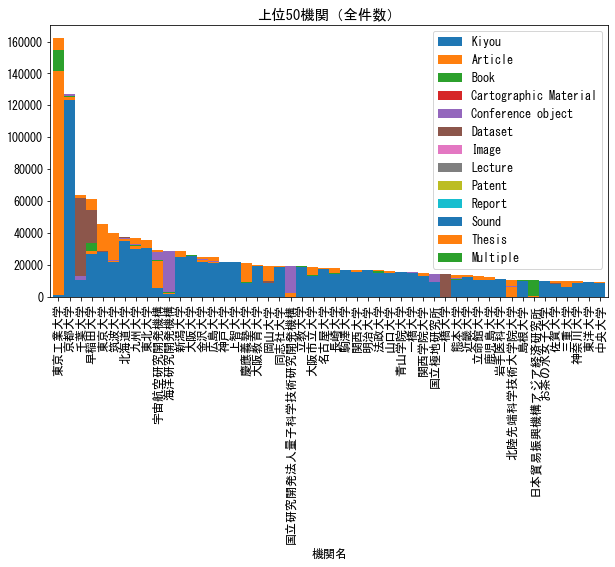
\includegraphics[width=8cm]{./picture/stack_all.png}
	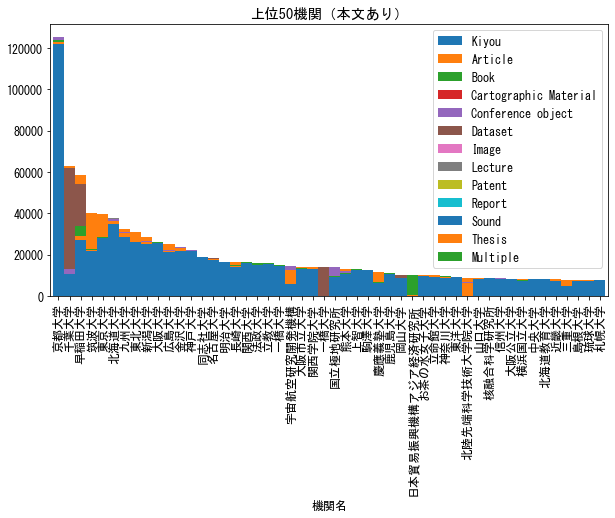
\includegraphics[width=8cm]{./picture/stack_honbun.png}
	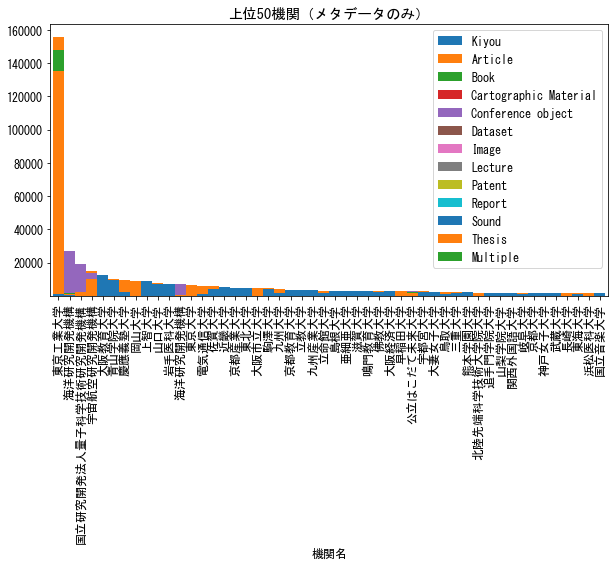
\includegraphics[width=8cm]{./picture/stack_sabun.png}
	\caption{コンテンツ数上位50機関で構成比率の積み上げグラフ}
	\ecaption{Stacked graph of composition ratios for the 
	top 50 institutions in terms of number of contents}
	\label{fig:stack1}
\end{figure}

図\ref{fig:percentage}のとおり、全体(n=792)を、
リポジトリごとのコンテンツ数の比率の高い順に並べてみると、
kiyou が多くを占め、かつkiyouが各リポジトリの中でほとんどを占めている機関が多いことが、
よりはっきりする。

\begin{figure}[h]
	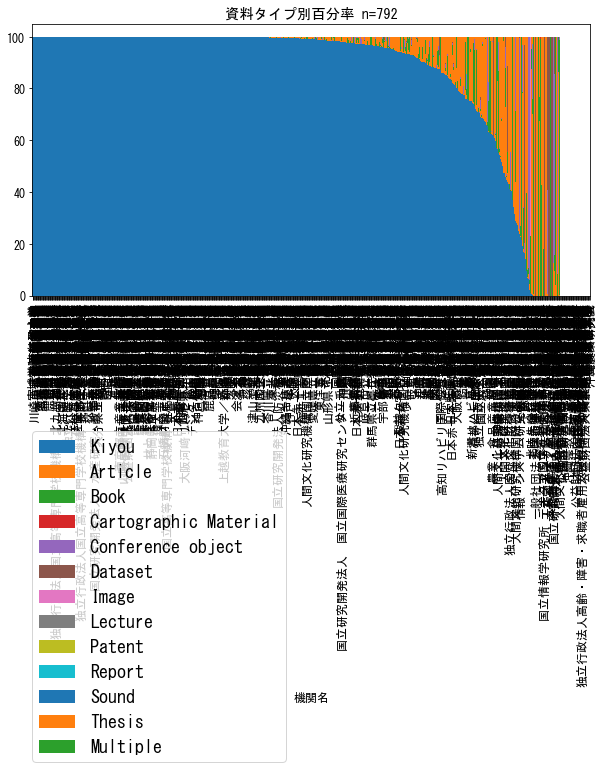
\includegraphics[width=8cm]{./picture/percentage_sort.png}
	\caption{資料タイプ別百分率}
	\ecaption{Stacked graph of composition ratios for the 
	top 50 institutions in terms of number of contents}
	\label{fig:percentage}
\end{figure}

実際には、資源タイプの内、Kiyou が90%を超えている機関が70%以上であった。

%3
\section{主成分分析}
\label{PCA}
前記、前処理の時点で、13次元のデータであり、それを可視化することは不可能である。
そこで、主成分分析を用いて情報をなるべく失うことなく2次元へと次元圧縮をし、データの可視化をおこなってみる。
主成分分析(principal component analysis)とは、
相関のある多数の変数から、相関のない少数で全体のばらつきを最もよく表す、
主成分と呼ばれる変数を合成する多変量解析の一手法で、
データの次元を削減するために用いられる。

%3.1
\subsection{主成分分析の前処理}
主成分分析の前処理として、標準偏差が小さい列を削除しておく。
標準偏差が小さい、ということは、全体のバラツキが小さいということ、
つまり、測定値の分布が平均値の周りに集まっているということを表している。

\begin{lstlisting}[language=Python,breaklines, caption=,label=df2205_all_dstd]
	std0 = (df2205_all_d.std(axis=0) > 1)
	df2205_all_dstd = df2205_all_d.loc[:, std0]
\end{lstlisting}

上記で、標準偏差が1より小さい列を削除することで、
Cartographic Material、Patent、Report、Sound、Multiple
の5列が削除されて、8列(8項目)になる。

ここで作成したデータフレームを

\begin{lstlisting}[language=Python,breaklines]
	df2205_all_dstd.describe()
\end{lstlisting}

にて確認すると、
表\ref{table:dstd}のとおりとなる。

25\%は第一四分位数、75\%は第三四分位数を表しており、kiyou(紀要)を除けば、
BookとThesisの2つに75\%は第三四分位数に数字があるのみであることが分かる。
四分位数とは、

“データを小さい方から並び替え、データの個数(サンプルサイズ)で4等分した時の
区切り点を四分位数と言う。\\
それぞれ25パーセンタイル(第一四分位数)、50パーセンタイル(中央値)、
75パーセンタイル(第三四分位数)とよばれる。”

\footnote{\url{https://bellcurve.jp/statistics/glossary/1919.html}}

であり、
紀要の場合全体の3/4の位置で129件あるが、図書は1/4の位置で2件、
学位論文は1/4の位置で20件しかないことが分かる。
紀要を除けば、他の資源タイプはゼロ件のリポジトリが圧倒的に多いことが推測できる。

このdf2205\_all\_dstdで箱ひげ図を描いてみると、図\ref{fig:box1}のようになる。

\begin{figure}[h]
	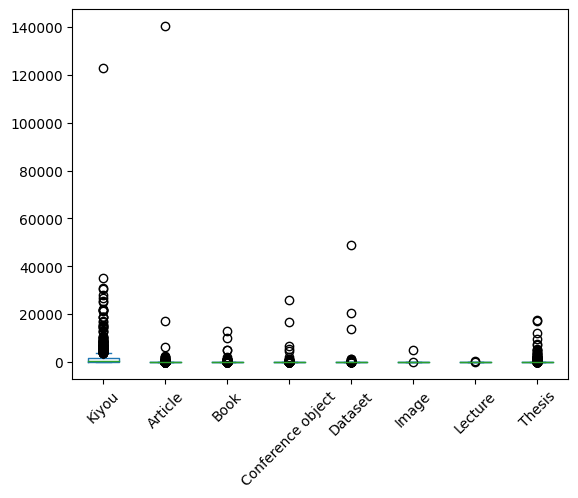
\includegraphics[width=8cm]{./picture/df2205alldstdboxplot.png}
	\caption{外れ値を除いた箱ひげ図}
	\ecaption{Single column figure with caption\\
		explicitly broken by $\backslash\backslash$.}
	\label{fig:box1}
\end{figure}

箱ひげ図は、データのばらつきをわかりやすく表現するための統計図であり、
一番上の線が最大値、一番下の線が最小値、中央の線が中央値などを示し、
丸は外れ値であり値に含まれない。
しかし、図 \ref{fig:box1}では、外れ値ばかりで、このままではばらつきなどが分からない。
そこで、それぞれ大きく外れているデータを以下で確認する。

\begin{lstlisting}[language=Python,breaklines]
	df2205_all_dstd[df2205_all_dstd['Kiyou']>40000]
	df2205_all_dstd[df2205_all_dstd['Article']>40000]
	df2205_all_dstd[df2205_all_dstd['Dataset']>40000]
\end{lstlisting}

結果は
表 \ref{table:outlier1}
のとおりとなった。

'Kiyou'は京都大学が、'Article'は東京工業大学が、'Dataset'は千葉大学が、
それぞれ大きく突出していることが分かる。
ここではデータの全体の感じをつかむため、この3機関を外し、さらにデータの多い'Kiyou'を外して
箱ひげ図を再度作成する。

図 \ref{fig:box2} のとおり、これでもあまり意味のある図にはならなかった。

\begin{figure}[h]
	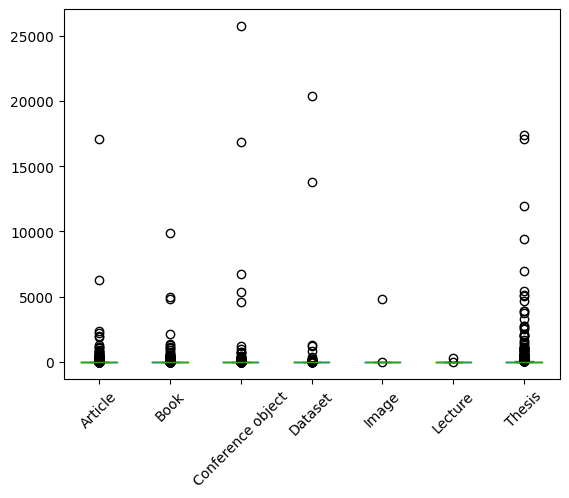
\includegraphics[width=8cm]{./picture/box2.png}
	\caption{外れ値を除いた箱ひげ図}
	\ecaption{Single column figure with caption\\
		explicitly broken by $\backslash\backslash$.}
	\label{fig:box2}
\end{figure}

%3.2
\subsection{特徴量の確認}

相関行列や散布図を用いて特徴量の分布などを確認する。

\begin{figure}[h]
	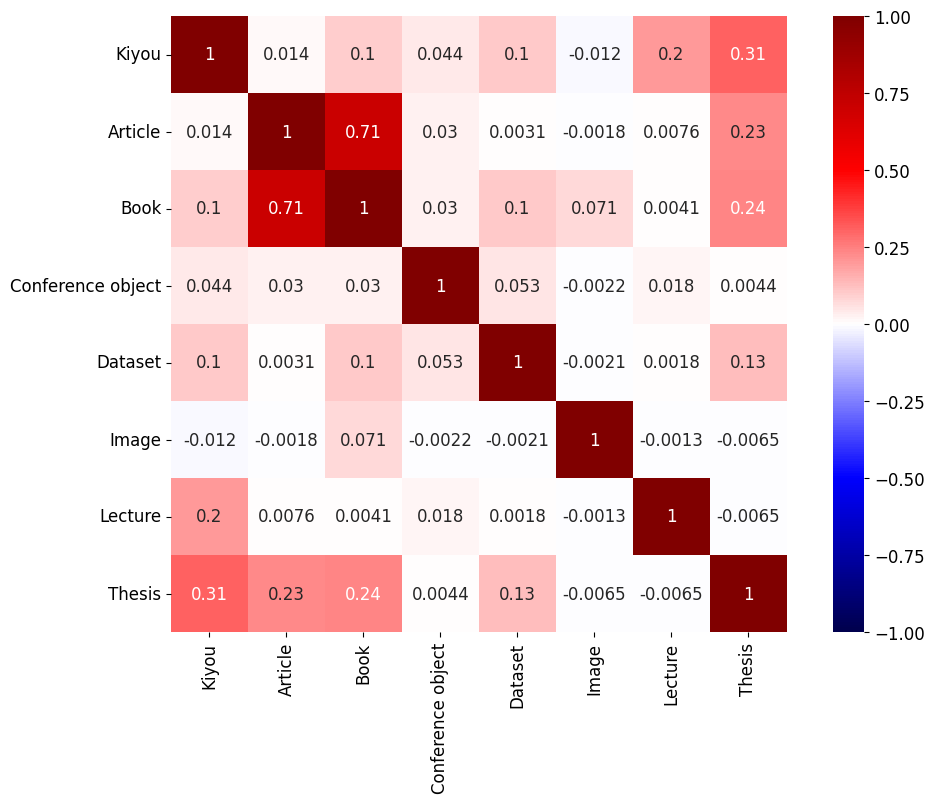
\includegraphics[width=8cm]{./picture/heatmap.png}
	\caption{相関行列のヒートマップ (相関係数の値あり)}
	\ecaption{Single column figure with caption\\
		explicitly broken by $\backslash\backslash$.}
	\label{fig:heatmap12}
\end{figure}

KiyouとArticleはあまり関係がなく、Kiyouと関係があるのはThesisであることが分かる。
これは、日本の機関リポジトリの一般的な印象とも合致する。

%3.3
\subsection{特徴量の標準化}

IRDBのデータから機関リポジトリの特徴を見るためには、量的な特徴を見るのが分かりやすいが、
機関リポジトリごとのコンテンツの量に差がありすぎるため、量以外の特徴がつかみにくい。
ここでは、分析の前処理として、特徴量を標準化する。
標準化はスケーリング(Feature Scaling)の一種で、特徴量間のスケールを変換することである。
特徴量間で異なるスケールを揃えるため、資源タイプごとに、元のデータの平均を0、
標準偏差が1となるように変換する。

\begin{lstlisting}[language=Python,breaklines]
	# 変数(特徴量)の標準化
	df2205_all_std = df2205_all_dstd.apply(lambda x: (x-x.mean())/x.std(), axis=0)
	# 結果を少数以下2桁で丸めて表示
	df2205_all_std.describe().round(2)
\end{lstlisting}

結果は \ref{table:std1} のとおり、
平均が0、標準偏差が1となるように変換されていることが分かる。

%5.4
\subsection{主成分分析}

以下で、主成分分析を実行する。

\begin{lstlisting}[language=Python,breaklines]
	from sklearn.decomposition import PCA
	# 主成分分析の実行
	pca = PCA()
	pca.fit(df2205_all_std)

	# データを主成分に変換
	pca_row = pca.transform(df2205_all_std)
\end{lstlisting}

次に、寄与率を求め、累積寄与率のグラフを書きます。
寄与率は、データの全情報の中で、各要素のもつ情報が占める割合を表し、
値が大きいほど相対的に説明力が高い主成分であることを示す。\\
累積寄与率は、寄与率を大きい順に順次足したもので、
主成分が全体の中でどれだけの割合を占めるかを示す。

\begin{lstlisting}[language=Python,breaklines]
# 寄与率を求める
pca_col = ["PC{}".format(x + 1) for x in range(len(df2205_all_std.columns))]
df_con_ratio = pd.DataFrame([pca.explained_variance_ratio_], columns = pca_col)
print(df_con_ratio)

# 累積寄与率を図示する
cum_con_ratio = np.hstack([0, pca.explained_variance_ratio_]).cumsum()
plt.plot(cum_con_ratio, 'D-')
plt.xticks(range(9))
plt.yticks(np.arange(0,1.05,0.05))
plt.grid()
plt.show()
\end{lstlisting}

以下のグラフによれば、第1主成分の寄与率は,0.23951 である
一般的には、累積寄与率が80%以上になる主成分数を採用して分析結果に用いることが多い
と言われているが、第2主成分までだと約40%であり、若干説明力は弱い。

\begin{figure}[h]
	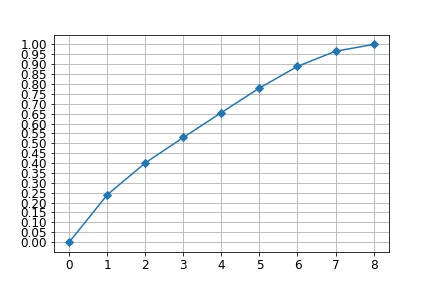
\includegraphics[width=8cm]{./picture/cumulative_contribution_ratio.png}
	\caption{累積寄与率}
	\ecaption{cumulative contribution ratio}
	\label{fig:umulative_contribution_ratio}
\end{figure}

第1主成分と第2主成分でプロットしてみる。

\begin{lstlisting}[language=Python,breaklines]
	# 第1主成分と第2主成分でプロットする
	import matplotlib.pyplot as plt
	plt.rcParams["font.family"] = "Meiryo" # "MS Gothic"
	plt.figure(figsize=(12, 12))
	plt.scatter(pca_row[:, 0], pca_row[:, 1], alpha=0.8)  # c=list(df2205_all_std.iloc[:, 0]))
	plt.grid()
	plt.xlabel("PC1")
	plt.ylabel("PC2")
	
	for k, v in pca_tokuten_0.iterrows():
		plt.annotate(k,xy=(v[0],v[1]),size=8)
	plt.show()
	\end{lstlisting}

\begin{figure}[h]
	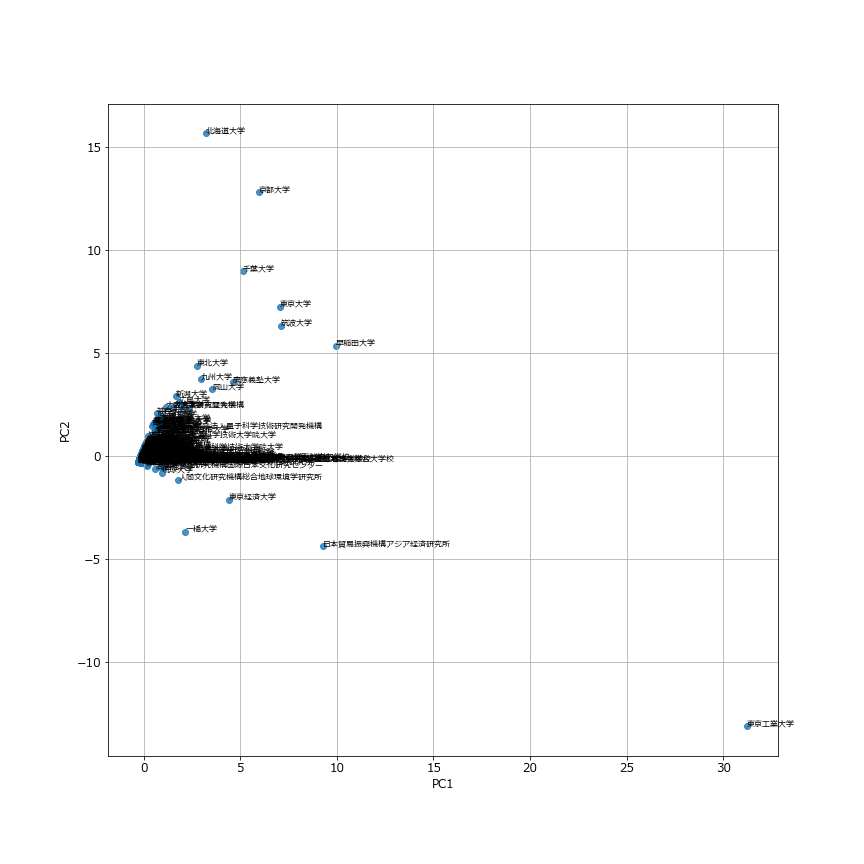
\includegraphics[width=8cm]{./picture/pc1pc2.png}
	\caption{第1主成分と第2主成分}
	\ecaption{first and second principal component}
	\label{fig:pc1pc2}
\end{figure}

グラフのとおり、第1主成分では東京工業大学が、
第2主成分では北海道大学や早稲田大学などが突出しており、
原点付近に集中しているため、文字が重なり真っ黒になってしまった。

次に、主成分に対する各変数の影響度合いを見るため、主成分負荷量を求める。
これにより,各主成分が何を意味しているかが分かりやすくなる。


\begin{lstlisting}[language=Python,breaklines]
	# 主成分負荷量を求める
	df_pca = pd.DataFrame(pca_row, columns = pca_col)
	df_pca_vec = pd.DataFrame(pca.components_, columns=df2205_all_std.columns,
		index=["PC{}".format(x + 1) for x in range(len(df_pca.columns))])
	print(df_pca_vec)
	
	# 主成分負荷量を図示する
	plt.figure(figsize=(6, 6))
	for x, y, name in zip(pca.components_[0], pca.components_[1], df2205_all_std.columns[0:]):
		plt.text(x, y, name)
	plt.scatter(pca.components_[0], pca.components_[1])
	plt.grid()
	plt.xlabel("PC1")
	plt.ylabel("PC2")
	plt.show()
\end{lstlisting}

\begin{figure}[h]
	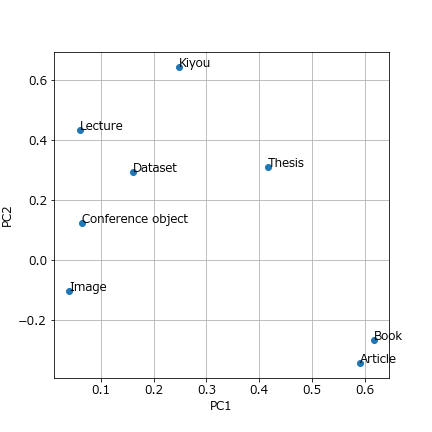
\includegraphics[width=8cm]{./picture/principal_component_loading.png}
	\caption{主成分負荷量}
	\ecaption{principal component loading}
	\label{fig:pcloading}
\end{figure}

図\ref{fig:pcloading}を見ると、第1主成分にはArticleとBookが、
第2主成分にはKiyouの影響が大きいことが分かり、
図\ref{fig:pc1pc2}で、
第1主成分が高い東京工業大学がArticleとBookの割合が高いこと、
第2主成分が高い北海道大学や早稲田大学がKiyouやLectureの割合が高いこと、
また、
図\ref{fig:heatmap12}の印象とも一致する。

図\ref{fig:pc1pc2}では、いわゆる外れ値が大きいので、外れ値を抜いて分析してみる。

\begin{lstlisting}[language=Python,breaklines]
	# 外れ値(例外的に、値が大きな機関)を削除する
	# nd配列pca_rowをDataFrameにする
	pca_row_df = pd.DataFrame(pca_row, index= list(df2205_all_std.index), columns=["PC{}".format(x + 1)
			for x in range(len(df2205_all_std.columns))])
	outlier = list(pca_row_df[pca_row_df[['PC1','PC2']] > 5].dropna(how='all').index)
	pca_row_df_o = pca_row_df.drop(outlier)
	print(outlier)
\end{lstlisting}

これにより、
'早稲田大学', '筑波大学', '東京工業大学', '東京大学', '京都大学', '日本貿易振興機構アジア経済研究所', '北海道大学', '千葉大学'
8機関が抽出され、日本の機関リポジトリとしては特徴的な機関であることが分かる。
さきほど同じように、第1主成分と第2主成分でプロットしてみる。
\begin{figure}[h]
	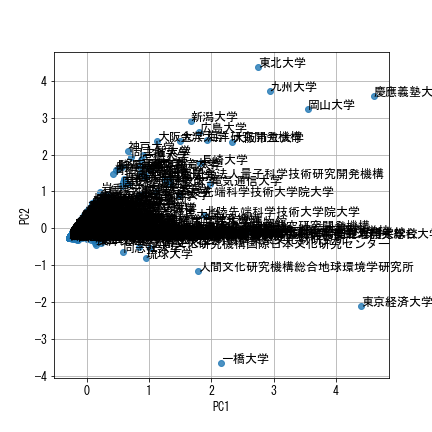
\includegraphics[width=8cm]{./picture/pc1pc2_outlier.png}
	\caption{第1主成分と第2主成分(外れ値を削除)}
	\ecaption{first and second principal component:outlier}
	\label{fig:pc1pc2_outlier}
\end{figure}

さらに同じように外れ値を抽出してみると、
'東京経済大学', '東北大学', '大阪大学', '大阪市立大学', '岡山大学', '新潟大学', '九州大学', '神戸大学', '慶應義塾大学', '金沢大学', '海洋研究開発機構', '宇宙航空研究開発機構', '一橋大学', '広島大学'
が特徴的な機関であることが分かった。

% %6
% \section{おわりに}

% 本稿では,

% \begin{acknowledgment}
% 	深謝する.
% \end{acknowledgment}

% \begin{thebibliography}{9}
% 	\bibitem{okumura}
% 	奥村晴彦:改訂第5版 \LaTeXe 美文書作成入門,
% 	技術評論社(2010).
	
% 	\bibitem{companion}
% 	Goossens, M., Mittelbach, F. and Samarin, A.: {\it The LaTeX Companion},
% 	Addison Wesley, Reading, Massachusetts (1993).
	
% 	\bibitem{book1}
% 	木下是雄:
% 	理科系の作文技術,
% 	中公新書(1981).
	
% 	\bibitem{book2}
% 	Strunk, W.J. and White, E.B.: {\it The Elements of Style, Forth Edition},
% 	Longman (2000).
	
% 	\bibitem{book3}
% 	Blake, G. and Bly, R.W.: {\it The Elements of Technical Writing},
% 	Longman (1993).
	
% 	\bibitem{book4}
% 	Higham, N.J.:
% 	{\it Handbook of Writing for the Mathematical Sciences},
% 	SIAM (1998).
	
% 	\bibitem{webpage1}
% 	情報処理学会論文誌ジャーナル編集委員会:
% 	投稿者マニュアル(オンライン),
% 	\urlj{http://www.ipsj.or.jp/journal/ submit/manual/j\_manual.html}%
% 	\refdatej{2007-04-05}.
	
% 	\bibitem{webpage2}
% 	情報処理学会論文誌ジャーナル編集委員会:
% 	べからず集(オンライン),
% 	\urlj{http://www.ipsj.or.jp/journal/\\ manual/bekarazu.html}%
% 	\refdatej{2011-09-15}.
	
% 	\end{thebibliography}
	
%============================
%--------------
\onecolumn

\begin{table}[tb]
	\caption{df2205\_all\_d.describe\(\)}
	\ecaption{df2205\_all\_d.describe\(\)}
	\label{table:alld}
	\hbox to\hsize{
		\begin{tabular}{p{0.7cm}p{0.7cm}|p{0.7cm}|p{1cm}|p{1cm}|p{1cm}|p{1cm}|p{1cm}|p{1cm}|p{1cm}|p{1cm}|p{1cm}|p{1cm}|p{1cm}}
		% \begin{tabular}{lrrrrrrrrrrrrr}

			&    Kiyou &  Article &    Book &  Cartographic Material &  Conference \par object &  Dataset &  Image &  Lecture &  Patent &  Report &  Sound &  Thesis &  Multiple \\\hline

			count &    792.0 &    792.0 &   792.0 &                  792.0 &              792.0 &    792.0 &  792.0 &    792.0 &   792.0 &   792.0 &  792.0 &   792.0 &     792.0 \\
			mean  &   2011.5 &    249.6 &    78.3 &                    0.0 &               93.8 &    112.7 &    6.1 &      0.4 &     0.0 &     0.0 &    0.0 &   217.2 &       0.0 \\
			std   &   5952.6 &   5051.3 &   643.6 &                    0.4 &             1151.1 &   1948.2 &  170.3 &     10.4 &     0.0 &     0.0 &    0.2 &  1201.0 &       0.0 \\
			min   &      0.0 &      0.0 &     0.0 &                    0.0 &                0.0 &      0.0 &    0.0 &      0.0 &     0.0 &     0.0 &    0.0 &     0.0 &       0.0 \\
			25\%   &    128.0 &      0.0 &     0.0 &                    0.0 &                0.0 &      0.0 &    0.0 &      0.0 &     0.0 &     0.0 &    0.0 &     0.0 &       0.0 \\
			50\%   &    482.5 &      0.0 &     0.0 &                    0.0 &                0.0 &      0.0 &    0.0 &      0.0 &     0.0 &     0.0 &    0.0 &     0.0 &       0.0 \\
			75\%   &   1517.0 &      0.0 &     2.0 &                    0.0 &                0.0 &      0.0 &    0.0 &      0.0 &     0.0 &     0.0 &    0.0 &    19.0 &       0.0 \\
			max   & 123440.0 & 140940.0 & 12907.0 &                   10.0 &            25743.0 &  48965.0 & 4792.0 &    294.0 &     0.0 &     0.0 &    7.0 & 17369.0 &       0.0 \\
			\end{tabular}
	}
\end{table}

% \twocolumn
%--------------

% \onecolumn

% 2段ぶちぬきで下方に図を表示する
\begin{figure}[tb]
	\label{fig:box100000000000000000000000000000}
	% \figref{fig:box1}
	\twocolfig{
		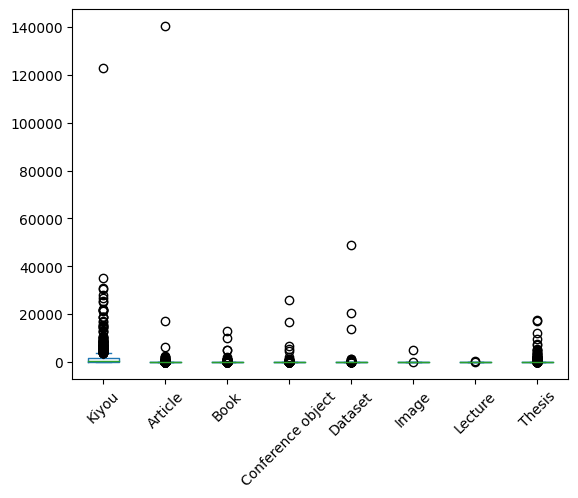
\includegraphics[width=12cm]{./picture/df2205alldstdboxplot.png}
	}
	\twocolcaption{df2205\_all\_dstdの箱ひげ図}
\end{figure}
% <大き目な図これ[b]だとボトムに図が表示される>



\begin{table}[tb]
	\caption{df2205\_all\_dstd.describe\(\)}
	\ecaption{df2205\_all\_dstd.describe\(\)}
	\label{table:dstd}
	\hbox to\hsize{\hfil
		\begin{tabular}{l|llllllll}\hline\hline
			      & 1Kiyou        & 2Article      & 2Book        & 5Conference object & 5Dataset     & 6Image      & 7Lecture   & 8Thesis      \\\hline
			count & 789.000000    & 789.000000    & 789.000000   & 789.000000         & 789.000000   & 789.000000  & 789.000000 & 789.000000   \\
			mean  & 1993.239544   & 249.602028    & 78.128010    & 93.576679          & 112.820025   & 6.076046    & 0.372624   & 218.742712   \\
			std   & 5919.979304   & 5044.485846   & 644.070755   & 1152.428752        & 1949.766679  & 170.599642  & 10.431092  & 1200.556001  \\
			min   & 0.000000      & 0.000000      & 0.000000     & 0.000000           & 0.000000     & 0.000000    & 0.000000   & 0.000000     \\
			25\%  & 129.000000    & 0.000000      & 0.000000     & 0.000000           & 0.000000     & 0.000000    & 0.000000   & 0.000000     \\
			50\%  & 487.000000    & 0.000000      & 0.000000     & 0.000000           & 0.000000     & 0.000000    & 0.000000   & 0.000000     \\
			75\%  & 1506.000000   & 0.000000      & 2.000000     & 0.000000           & 0.000000     & 0.000000    & 0.000000   & 20.000000    \\
			max   & 122935.000000 & 140481.000000 & 12883.000000 & 25743.000000       & 48965.000000 & 4792.000000 & 293.000000 & 17369.000000 \\\hline
		\end{tabular}\hfil}
\end{table}


\begin{table}[tb]
	\caption{df2205\_all\_dstd.describe\(\)}
	\ecaption{df2205\_all\_dstd.describe\(\)}
	\label{table:outlier1}
	\hbox to\hsize{\hfil
		\begin{tabular}{l|llllllll}\hline\hline
			                & 1Kiyou & 2Article & 2Book & 5Conference object & 5Dataset & 6Image & 7Lecture & 8Thesis \\\hline
			京都大学'Kiyou'     & 122935 & 1460     & 940   & 1147               & 254      & 0      & 0        & 0       \\
			東京工業大学'Article' & 828    & 140481   & 12883 & 0                  & 11       & 0      & 0        & 7572    \\
			千葉大学'Dataset'   & 10557  & 91       & 134   & 2065               & 48965    & 0      & 0        & 1970    \\\hline
		\end{tabular}\hfil}
\end{table}

\begin{table}[tb]
	\caption{df2205\_all\_dstd.describe\(\)}
	\ecaption{df2205\_all\_dstd.describe\(\)}
	\label{table:std1}
	\hbox to\hsize{\hfil
		\begin{tabular}{l|llllllll}\hline\hline
			      & 1Kiyou & 2Article & 2Book  & 5Conference object & 5Dataset & 6Image & 7Lecture & 8Thesis \\\hline
			count & 789.00 & 789.00   & 789.00 & 789.00             & 789.00   & 789.00 & 789.00   & 789.00  \\
			mean  & -0.00  & -0.00    & 0.00   & 0.00               & 0.00     & 0.00   & -0.00    & 0.00    \\
			std   & 1.00   & 1.00     & 1.00   & 1.00               & 1.00     & 1.00   & 1.00     & 1.00    \\
			min   & -0.34  & -0.05    & -0.12  & -0.08              & -0.06    & -0.04  & -0.04    & -0.18   \\
			25\%  & -0.31  & -0.05    & -0.12  & -0.08              & -0.06    & -0.04  & -0.04    & -0.18   \\
			50\%  & -0.25  & -0.05    & -0.12  & -0.08              & -0.06    & -0.04  & -0.04    & -0.18   \\
			75\%  & -0.08  & -0.05    & -0.12  & -0.08              & -0.06    & -0.04  & -0.04    & -0.17   \\
			max   & 20.43  & 27.80    & 19.88  & 22.26              & 25.06    & 28.05  & 28.05    & 14.29   \\\hline
		\end{tabular}\hfil}
\end{table}

\twocolumn


%====================

\end{document}
